\documentclass{beamer}
\mode<presentation> {
    \usetheme{Copenhagen} \usecolortheme{whale}
    }
\usepackage{graphicx}
\usepackage{multicol}
\usepackage{subfig}

\setbeamersize{text margin left=3mm,text margin right=5mm }
\geometry{paperwidth=650pt, paperheight=400pt}
\usepackage{verbatim}
\graphicspath{{Images/}}
\title[Assignments 7]{Pendolo Inverso}
\author{Lorenzo Rossi Matricola: 0301285}
\begin{document}
\begin{frame}
	\titlepage{}
\end{frame}
\begin{frame}
	\begin{columns}[t]
		\begin{column}{.5\textwidth}
			\tableofcontents[sections={1-5}] % chktex 8
		\end{column}
		\hspace{-1cm}
		\begin{column}{.5\textwidth}
			\tableofcontents[sections={6-11}] % chktex 8
		\end{column}
	\end{columns}
\end{frame}
\begin{frame}
	\frametitle{Formulazione del Sistema}
	\section{A0 - Formulazione del sistema}% chktex 8
	Noti: \(M=1 kg,L=1m,F=1\frac{Kg}{s},g=9.81\frac{m}{s^2}\)\newline
	\begin{tabular}{c|c} % chktex 44
		\begin{minipage}{0.55\textwidth}
			\begin{equation*}
				\begin{cases}
					M\ddot{s}+F\dot{s}-\mu=d_{1} \\
					\ddot{\phi}-\frac{g}{L}\sin{(\phi)}+\frac{1}{L}\ddot{s}\cos{(\phi)}=0
				\end{cases}
			\end{equation*}
			Esplicitando \(\ddot{s},\ddot{\phi}\) si ottiene;\small
			\begin{equation*}
				\begin{cases}
					\ddot{s}=-\frac{F}{M}\dot{s}+\frac{1}{M}\mu+\frac{1}{M}d_1 \\
					\ddot{\phi}=\frac{g}{L}\sin{(\phi)}-\frac{1}{L}\ddot{s}\cos{(\phi)}=\frac{g}{L}\sin{(\phi)}+\frac{1}{L}(\frac{F}{M}\dot{s}-\frac{1}{M}\mu-\frac{1}{M}d_1)
				\end{cases}
			\end{equation*}
			Sia:
			\begin{equation*}
				x=\begin{bmatrix}
					x_{1} & x_{2} & x_{3} & x_{4}
				\end{bmatrix}^{T}=\begin{bmatrix}s & \dot{s} & \phi & \dot{\phi}
				\end{bmatrix}^{T}
			\end{equation*}
			\begin{equation*}
				u=\begin{bmatrix}
					u_{1} & u_{2}
				\end{bmatrix}^{T}=\begin{bmatrix}\mu & d_{1}
				\end{bmatrix}^{T}
			\end{equation*}
		\end{minipage} &
		\begin{minipage}{0.40\textwidth}
			Si ottiene il sistema finale:\small
			\begin{equation*}
				\begin{cases}
					\dot{x_{1}}=x_2                                                 \\
					\dot{x_{2}}=-\frac{F}{M}x_{2}+\frac{1}{M}u_{1}+\frac{1}{M}u_{2} \\
					\dot{x_{3}}=x_{4}                                               \\
					\dot{x_{4}}=\frac{g}{L}\sin{(x{3})}+\frac{1}{L}(\frac{F}{M}x_{2}-\frac{1}{M}u_{1}-\frac{1}{M}u_{2})\cos{(x{3})}
				\end{cases}
			\end{equation*}
		\end{minipage}
	\end{tabular}
\end{frame}
\begin{frame}
	\frametitle{A1 - Punti Equilibrio}% chktex 8
	\section{A1 - Punti di Equilibrio}% chktex 8
	\textbf{Calcolare tutte i punti di equilibrio del sistema per \(\mu = d_{1}{(t)} = 0\)}
	Si impone \(\dot{x}=\textbf{0}\):
	\begin{equation*}
		\begin{cases}
			\dot{x_{1}}=0 \\
			\dot{x_{2}}=0 \\
			\dot{x_{3}}=0 \\
			\dot{x_{4}}=0
		\end{cases}
		\rightarrow
		\begin{cases}
			0=x_{2} \\
			0=0     \\
			0=x_{4} \\
			0=\sin{x_{3}}
		\end{cases}
		\rightarrow
		\begin{cases}
			s:x_{1}\in\mathbb{R}        \\
			\dot{s}:x_{2}=0             \\
			\phi:x_{3}=0 \lor x_{3}=\pi \\% chktex 21
			\dot{\phi}:x_{4}=0
		\end{cases}
	\end{equation*}
	In particolare, si ha un punto di equilibrio nei casi in cui:\begin{itemize}
		\item Le velocità del carrello e del pendolo sono nulle;
		\item Il pendolo è perpendicolare al piano.
		\item Qualisiasi posizione del piano su cui si muove il carrello è un punto di equilibrio.
	\end{itemize}
\end{frame}
\begin{frame}
	\frametitle{A2 - Linearizzazione del sistema} % chktex 8
	\section{A2 - Linearizzazione del sistema} % chktex 8
	\textbf{Scrivere le equazioni del sistema linearizzato attorno al punto di equilibrio \(\phi=s=\dot{\phi}=\dot{s}=0\)}
	Per ottenere la linearizzazione occorre imporre che:\begin{equation*}
		A_{lin}=\nabla_{x}f(x,u)\lvert_{x=0,u=0}\quad
		B_{lin}=\nabla_{u}f(x,u)\lvert_{x=0,u=0}\quad
	\end{equation*}
	Quindi, effettuando le derivate si giunge a:
	\begin{equation*}
		A_{lin}=\begin{bmatrix}
			0 & 1            & 0           & 0 \\
			0 & -\frac{F}{M} & 0           & 0 \\
			0 & 0            & 0           & 1 \\
			0 & \frac{F}{LM} & \frac{g}{L} & 0
		\end{bmatrix}
		\quad B_{lin}=\begin{bmatrix}
			0 & 0 \\\frac{1}{M}&\frac{1}{M}\\0&0\\-\frac{1}{LM}&-\frac{1}{LM}
		\end{bmatrix}
	\end{equation*}
	\begin{equation*}
		\dot{\tilde{x}}=A_{lin}\tilde{x}+B_{lin}u
	\end{equation*}
\end{frame}
\begin{frame}
	\frametitle{A3 - Forma standard nello spazio di stato}% chktex 8
	\section{A3 - Forma standard nello spazio di stato}% chktex 8
	\textbf{Scrivere il sistema lineare nella forma:\begin{equation*}
			\dot{x}=Ax+Bu+PD,\quad y=Cx
		\end{equation*}}
	Siano:\begin{equation*}
		x(t)=\begin{bmatrix}
			s(t) & \dot{s(t)} & \phi(t) & \dot{\phi(t)}
		\end{bmatrix}^{T}\quad u(t)=\mu(t)\quad y(t)=\begin{bmatrix}
			s(t) & \phi(t)
		\end{bmatrix}^{T}
	\end{equation*}
	Quindi:\small
	\begin{equation*}
		\dot{x}=\begin{bmatrix}
			0 & 1            & 0           & 0 \\
			0 & -\frac{F}{M} & 0           & 0 \\
			0 & 0            & 0           & 1 \\
			0 & \frac{F}{LM} & \frac{g}{L} & 0
		\end{bmatrix}x+\begin{bmatrix}
			0 \\\frac{1}{M}\\0\\-\frac{1}{LM}
		\end{bmatrix}u+\begin{bmatrix}
			0 \\\frac{1}{LM}\\0\\-\frac{1}{LM}
		\end{bmatrix}d_{1}\quad y=\begin{bmatrix}
			1 & 0 & 0 & 0 \\0&0&1&0
		\end{bmatrix}x
	\end{equation*}
\end{frame}
\begin{frame}
	\frametitle{A4 - Controllabilità}% chktex 8
	\section{A4 - Controllabilità}% chktex 8
	\textbf{Mostra che la coppia \((A,B)\) è controllabile}
	A tempo continuo vale che:
	\begin{block}{}
		\((A,B) \) controllabile \(\Longleftrightarrow \) \((A,B) \) raggiungibile  \(\Longleftrightarrow
		rank{(R)}=n \quad n=\dim{(A)},\quad R= \begin{bmatrix}
			B\ AB\ \dots A^{n-1}B
		\end{bmatrix}\)
	\end{block}
	\begin{equation*}
		rank(R)=rank\left(\begin{bmatrix}
			0             & \frac{1}{M}      & -\frac{F}{M^2}                         & \frac{F^{2}}{M^{3}}                        \\
			\frac{1}{M}   & -\frac{F}{M^2}   & \frac{F^{2}}{M^{3}}                    & -\frac{F^{3}}{M^{4}}                       \\
			0             & -\frac{1}{LM}    & \frac{F}{LM^{2}}                       & -\frac{g}{L^{2}M}-\frac{F^{2}}{LM^{3}}     \\
			-\frac{1}{LM} & \frac{F}{LM^{2}} & -\frac{g}{L^{2}M}-\frac{F^{2}}{LM^{3}} & \frac{Fg}{L^{2}M^{2}}+\frac{F^{3}}{LM^{4}} \\
		\end{bmatrix}\right)=4
	\end{equation*}
	La coppia \((A,B) \) è controllabile.
\end{frame}
\begin{frame}
	\frametitle{A5 - Problema di Regolazione}% chktex 8
	\section{A5 - Problema di Regolazione}% chktex 8
	Per formulare un problema di regolazione si procede nel seguente modo:
	\begin{equation*}
		\dot{d_{1}}=0\rightarrow \dot{d_{1}}=S_{1}d_{1}\text{ con} S_{1}=\begin{bmatrix}
			0
		\end{bmatrix}\Longleftrightarrow d_{1}(t)=d_{1}(0),\forall t\geq 0
	\end{equation*}
	\begin{equation*}
		d_{2}=\alpha\sin{(\omega t)}\rightarrow \dot{\overline{d_2}}=S_{2}\overline{d_{2}}\quad S_{2}=\begin{bmatrix}
			0       & \omega \\
			-\omega & 0
		\end{bmatrix},\overline{d_{2}}(0)=\begin{bmatrix}
			0 \\\alpha
		\end{bmatrix}\Rightarrow d_{2}(t)=\begin{bmatrix}
			1 & 0
		\end{bmatrix}\overline{d_{2}}(t)
	\end{equation*}
	Con l'introduzione del segnale \(d_{3}(t)\) è possibile esprimere i segnali esogeni tramite:
	\begin{equation*}
		\dot{d}=Sd=\begin{bmatrix}
			0 & 0 & 0 \\ 0&0&\omega \\0&-\omega & 0
		\end{bmatrix}d\quad d(t)=\begin{bmatrix}
			d_{1}(t) \\d_{2}(t)\\d_{3}(t)
		\end{bmatrix},d(0)=\begin{bmatrix}
			const \\0\\\alpha
		\end{bmatrix}
	\end{equation*}
	Infine, definendo \(e(t)=x{1}(t)-d_(t)=s(t)-d_{2}(t)=s(t)-\alpha\sin{(\omega t)}\), si riscrive il sistema A3.

\end{frame}
\begin{frame}
	\frametitle{A5.1 - Problema di Regolazione}% chktex 8
	Il nuovo sistema viene descritto dalle seguenti equazioni:
	\begin{equation*}
		\begin{cases}
			\dot{x}=Ax+Bu+Pd \\
			y=Cx             \\
			e=C_{e}x+Qd      \\
			\dot{d}=Sd
		\end{cases}
	\end{equation*}
	In cui:\begin{equation*}
		A=\begin{bmatrix}
			0 & 1            & 0           & 0 \\
			0 & -\frac{F}{M} & 0           & 0 \\
			0 & 0            & 0           & 1 \\
			0 & \frac{F}{LM} & \frac{g}{L} & 0
		\end{bmatrix},\quad B=\begin{bmatrix}
			0 \\\frac{1}{M}\\0\\-\frac{1}{LM}
		\end{bmatrix}\quad P=\begin{bmatrix}
			0 & 0 & 0 \\\frac{1}{LM}&0&0\\0&0&0\\-\frac{1}{LM}&0&0
		\end{bmatrix}
		C=\begin{bmatrix}
			1 & 0 & 0 & 0 \\0&0&1&0
		\end{bmatrix},\quad C_{e}=\begin{bmatrix}
			1 & 0 & 0 & 0
		\end{bmatrix}\quad S=\begin{bmatrix}
			0 & 0 & 0 \\ 0&0&\omega \\0&-\omega & 0
		\end{bmatrix}
	\end{equation*}
	\begin{center}
		\begin{equation*}
			Q=\begin{bmatrix}
				0 & -1 & 0
			\end{bmatrix}
		\end{equation*}
	\end{center}
\end{frame}
\begin{frame}
	\frametitle{A6 - Legge di controllo a full information}% chktex 8
	\section{A6 - Legge di controllo a full information}% chktex 8
	\textbf{Consideriamo il problema di regolazione A5. Mostra che il problema è risulubile tramite una legge di controllo a full information}
	In un problema di regolazione a full information vogliamo determinare una legge di controllo \(u=Kx+Ld,L=\Gamma -K\Pi \) tale che:\begin{itemize}
		\item \textbf{S}: Il sistema \(\dot{x}=(A+BK)x\) sia asintoticamente stabile;
		\item \textbf{R}: Tutte le traiettorie del sistema:\begin{equation*}
			      \begin{cases}
				      \dot{x}=(A+BK)x+(BL+P)d \\
				      y=Cx                    \\
				      e=C_{e}x+Qd             \\
				      \dot{d}=Sd
			      \end{cases}
		      \end{equation*}
		      sono tali che \(\lim_{t\rightarrow \infty}e(t)=0\).
	\end{itemize}
	Per il teorema del problema di regolazione a full information FBI, esiste una legge di controllo a full information se e solo se \(\exists \Pi ,\Gamma \) tale che siano soddisfatte le equazioni:\(\Pi S= A\Pi +B\Pi+P\quad 0=C\Pi+Q\).
	Inoltre, dal lemma di Hautus si ha che il teorema FBI è soddisfatto \(\forall P,Q\) se e solo se:\begin{equation*}
		rank\left(\begin{bmatrix}
			sI-A & B \\C&0
		\end{bmatrix}\right)=n+p\quad \forall s\in \sigma(S)
	\end{equation*}
\end{frame}
\begin{frame}
	\frametitle{A6.1 - Legge di controllo a full information}% chktex 8
	Quindi:\begin{equation*}
		rank\left(\begin{bmatrix}
				s & -1            & 0            & 0  & 0             \\
				0 & s+\frac{F}{M} & 0            & 0  & \frac{1}{M}   \\
				0 & 0             & s            & -1 & 0             \\
				0 & -\frac{F}{LM} & -\frac{g}{L} & s  & -\frac{1}{LM} \\
				1 & 0             & 0            & 0  & 0
			\end{bmatrix}\right)=5,\forall{s}\in\sigma(S)\Longrightarrow \text{Equazioni FBI rispettate}
	\end{equation*}
\end{frame}
\begin{frame}
	\frametitle{A7 - Legge di controllo in feedback dall'errore}% chktex 8
	\section{A7 - Legge di controllo in feedback dall'errore}% chktex 8
	Sia \(e_{0}=\begin{bmatrix}
		e \\\phi
	\end{bmatrix}=\begin{bmatrix}
		s-d_{2} \\\phi
	\end{bmatrix}=Cx+Q_{0}d\) con \(Q_{0}=\begin{bmatrix}
		- & Q & - \\0&0&0
	\end{bmatrix}=\begin{bmatrix}
		0 & -1 & 0 \\0&0&0
	\end{bmatrix}\). Questo segnale è necessario alla realizzazione dell'osservatore che produce le stime \(\zeta(t),\delta(t)\), rispettivamente di \(x(t)\) e\( d(t)\), necessarie alla generazione del controllo \(u(t)\). Quindi il controllore dinamico risultante è del tipo:
	\begin{equation*}
		\begin{cases}
			\dot{\chi}=F\chi+Ge_{0} \\
			u=H\chi
		\end{cases}\quad
		\chi=\begin{bmatrix}
			\zeta \\ \delta
		\end{bmatrix}
	\end{equation*}
	Inoltre, deve essere tale che:
	\begin{itemize}
		\item \textbf{S}:\begin{equation*}
			      \begin{cases}
				      \dot{x}=Ax+BH\chi \\
				      \dot{\chi}=F\chi+GCx
			      \end{cases}
		      \end{equation*}\\ asintoticamente stabile;
	\item \textbf{R}:
	\begin{tabular}{c c}
		\(\begin{aligned}
			\begin{cases}
				\dot{x}=Ax+BH\chi+Pd          \\
				\dot{\chi}=F\chi+G(Cx+Q_{0}d) \\
				y=Cx                          \\
				e=C_{e}x+Qd                   \\
				\dot{d}=Sd
			\end{cases}
		\end{aligned}\) &
		\(\begin{aligned}
			F=\begin{bmatrix}
				A+G_{1}C+BK & P+G_{1}Q_{0}+BL \\
				G_{2}C      & S+G_{2}Q_{0}
			\end{bmatrix}\quad H=\begin{bmatrix}
				K & L
			\end{bmatrix}\quad G=-\begin{bmatrix}
				G_{1} \\G_{2}
			\end{bmatrix}\quad L=\Gamma-K\Pi
		\end{aligned}\)
		\end{tabular}\\
	con le traiettorie \(\lim_{t\rightarrow \infty }e(t)=0 \)
\end{itemize}
\end{frame}
\begin{frame}
	\frametitle{A7.1 - Legge di controllo in feedback dall'errore }% chktex 8
	Per la realizzazione dell'osservatore occorre verificare che la coppia \(A_{0},C_{0}=\left(\begin{bmatrix}
		A&P\\0&S
	\end{bmatrix},\begin{bmatrix}
		C&Q_{0}
	\end{bmatrix}\right)\). In particolare:
	\begin{block}{}
		\begin{center}
			\((A,C)\) osservabile \(\Longleftrightarrow rank(O)=n\) con \(n=\dim{(A_{0})}=7,O=\begin{bmatrix}
				C_{0}\\C_{0}A_{0}\\\vdots \\C_{0}A_{0}^{n-1}
			\end{bmatrix}\)
		\end{center}
	\end{block}
	Nel nostro caso \(rank(O)=7\Rightarrow (A_{0},C_{0})\) è osservabile. Inoltre, bisogna soddisfare i requisiti di regolazione. Per cui, definito \(e=C_{e}x+Qd=s-d_{2}\) si ha che:
	\begin{itemize}
		\item Dal teorema FBI:\(\exists{F,G,H}\)tali che si rispettino le condizioni \textbf{S},\textbf{R} se e solo se:\begin{equation*}
			\exists{\Gamma,\Pi}:\begin{cases}
				\Pi S= A\Pi +B\Pi+P\\
				 0=C\Pi+Q
			\end{cases}
		\end{equation*}
		\item Dal lemma di Hautus:\begin{equation*}
			\exists{\Gamma,\Pi}:\begin{cases}
				\Pi S= A\Pi +B\Pi+P\\
				 0=C\Pi+Q
			\end{cases}\forall P,Q\Longleftrightarrow rank\left(\begin{bmatrix}
				sI-A&B\\C_{e}&0
			\end{bmatrix}\right)=n+p=5\forall s\in\sigma(S)
		\end{equation*}
	\end{itemize}
\end{frame}
\begin{frame}
	\frametitle{B1 - Legge di controlo full information A5}% chktex 8
	\section{B1 - Legge di controlo full information A5}% chktex 8
	La legge di controlo full information si ottiene dalle equazioni FBI.In particolare, si ottiene che:% chktex 13
	\begin{equation*}
		\Pi=\begin{bmatrix}
			0&1&0\\0&0&\omega \\0&-\frac{\omega^{2}}{L\omega^{2}+g}&0\\0&0&-\frac{\omega^{3}}{L\omega^{2}+g}
		\end{bmatrix}\quad \Gamma=\begin{bmatrix}
			-1&-M\omega^{2}&F\omega
		\end{bmatrix}
	\end{equation*}
	Inoltre, la legge di controllo \(u=Kx+(\Gamma-K\Pi )d\) viene scelta con \(K\) tale che la matrice \(A+BK\) abbia gli autovalori desiderati per cui si ottiene stabilità asintotica. L'assegnazione degli autovalori può essere effettuata tramite la formula di Ackermann o di Mitter.
\end{frame}
\begin{frame}
	\frametitle{B2+B3 - Simulazioni \(\omega=0.1\): Lineare e Non Lineare}% chktex 8
	\section{B2+B3 - Simulazioni}% chktex 8
	\begin{tabular}{cc}
		\begin{minipage}{0.45\textwidth}
			\begin{equation*}
				\sigma (A+BK)=(-1.5,-1.2,-1,-0.8)
			\end{equation*}
			Nel caso del modello linearizzato, l'obiettivo di regolazione è perfetamente raggiunto:
			\begin{itemize}
				\item \(d_{1}\) non influisce su y poiché bilanciata dal controllo \(u\);
				\item Il controllo \(u\) è composto da:
				\begin{itemize}
					\item Contributo per la regolazione di \(e\);
					\item Contributo che contrasta il disturbo \(d_{1}\);
				\end{itemize}
			\end{itemize}
			Applicando lo stesso controllo al modello non lineare, si raggiunge l'obiettivo di regolazione in maniera approssimata. Sono presenti a regime delle oscillazioni contenute coerenti al disturbo \(d_{2}\).
			Il disturbo \(d_{1}\) non influisce su \(y\) e viene bilanciato dal controllo u.
		\end{minipage}
		&
		\begin{minipage}{0.45\textwidth}
			\begin{figure}
				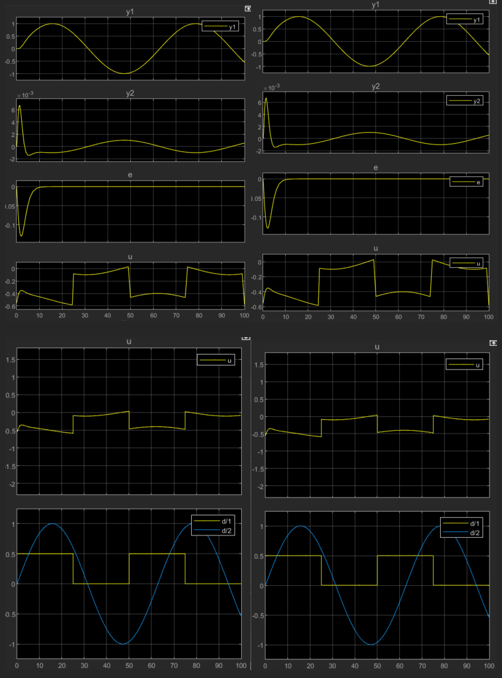
\includegraphics[scale=0.55]{2022-06-20-13-22-43.png}% chktex 8
			\end{figure}
		\end{minipage}
	\end{tabular}
\end{frame}
\begin{frame}
	\frametitle{B4 - Simulazione \(\omega= 1 \): Lineare e Non Lineare}% chktex 8
	\section{B4 - Simulazioni}% chktex 8
	\begin{tabular}{cc}
		\begin{minipage}{0.45\textwidth}
			\begin{equation*}
				\sigma(A+BK)=(-1.5,-1.2,-1,-0.8)
			\end{equation*}
			L'aumentare del disturbo comporta un allontanamento dal punto di equilibrio \(x=0\) poiché la regolazione avviene rispetto ad un segnale che varia più velocemente.
			Questo comporta che il modello linearizzato approssima in maniera meno accurata il modello non lineare con un controllo meno efficace.\newline A regime è possibile notare che l'andamento dell'errore presenta oscillazioni più elevate.
		\end{minipage}
		&
		\begin{minipage}{0.45\textwidth}
			\begin{figure}
				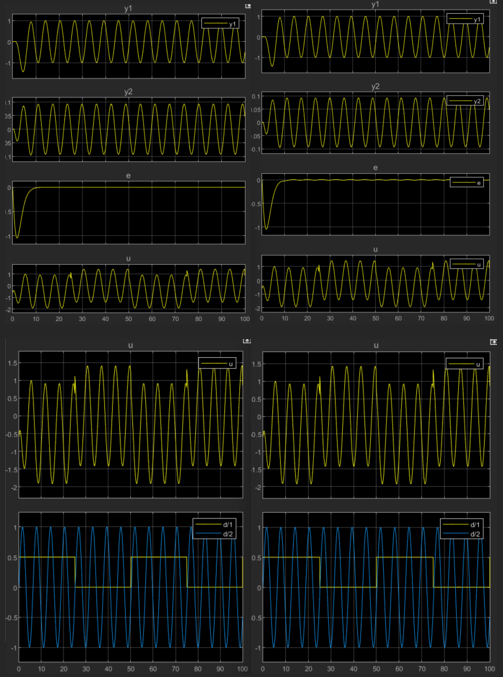
\includegraphics[scale=0.55]{2022-06-20-13-25-34.png}% chktex 8
			\end{figure}
		\end{minipage}
	\end{tabular}
\end{frame}
\begin{frame}
	\frametitle{B4 - Simulazione \(\omega=10 \): Lineare e Non linerare}% chktex 8
	\begin{tabular}{cc}
		\begin{minipage}{0.45\textwidth}
			\begin{equation*}
				\sigma(A+BK)=(-1.5,-1.2,-1,-0.8)
			\end{equation*}
			In questo caso, non si ragginge l'obiettivo di regolazion.\newline Il conrollore diventa quindi inadeguato ed il sistema complessivo risulta instabile causanto la divergenza dell'errore di inseguimento.\newline
			Inoltre, rimangono inalterate le prestazioni del modello linearizzato ma che non rispetta il comportamento del sistema reale.
		\end{minipage}
		&
		\begin{minipage}{0.45\textwidth}
			\begin{figure}
				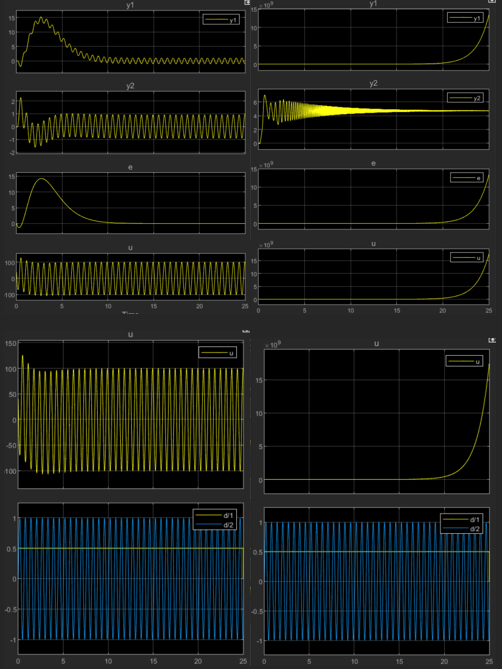
\includegraphics[scale=0.55]{2022-06-20-13-27-00.png}% chktex 8
			\end{figure}
		\end{minipage}
	\end{tabular}
\end{frame}
\end{document}